\documentclass[12pt, a4paper]{article}

\usepackage[utf8]{inputenc}
\usepackage[russian]{babel}

\usepackage{graphicx}
\usepackage{amsfonts}
\usepackage{amsmath}
\usepackage{cmap}
\usepackage[hidelinks]{hyperref}
\usepackage{epstopdf}
\usepackage{cite}
\usepackage{indentfirst}
\usepackage{listings}
\usepackage{xcolor}
\usepackage{array}
\usepackage{float}

\usepackage[left=2cm,right=1cm,
top=2cm,bottom=2cm,bindingoffset=0cm]{geometry}

\graphicspath{{images/}}

\definecolor{codegreen}{rgb}{0,0.6,0}
\definecolor{codegray}{rgb}{0.5,0.5,0.5}
\definecolor{codepurple}{rgb}{0.58,0,0.82}
\definecolor{backcolour}{RGB}{185,185,185}

\lstdefinestyle{bashstyle}{
	language=bash,
	backgroundcolor=\color{backcolour},   
	commentstyle=\color{codegreen},
	keywordstyle=\color{magenta},
	numberstyle=\tiny\color{codegray},
	stringstyle=\color{codepurple},
	basicstyle=\ttfamily\footnotesize,
	breakatwhitespace=false,         
	breaklines=true,                 
	captionpos=b,                    
	keepspaces=true,                                  
	showspaces=false,                
	showstringspaces=false,
	showtabs=false,                  
	tabsize=2,
	emph={make, cmake, mkdir, ctest},
	emphstyle = {\color{magenta}},
}

\lstset{style=bashstyle}


\begin{document}
	
\thispagestyle{empty}

\begin{center}
	\ \vspace{-3cm}
	
	
\includegraphics[width=0.5\textwidth]{msu-eps-converted-to.pdf}\\
	{Московский государственный университет имени М. В. Ломоносова}\\
	Факультет вычислительной математики и кибернетики\\
	Кафедра вычислительных методов
	
	\vspace{6cm}
	
	{\Large \bfseries Построение разреженной матрицы и решение СЛАУ}
	
	\vspace{1cm}
	
	{\large Параллельные высокопроизводительные вычисления}
\end{center}

\vfill

\begin{flushright}
	\textbf{выполнил:}\\
	Петров Т.\,П. \\
	группа 504
\end{flushright}

\vfill

\begin{center}
	15 ноября \\
	Москва, 2024
\end{center}

\enlargethispage{2\baselineskip}

\newpage

\tableofcontents

\newpage

\section{Описание задания и программной реализации}
\subsection{Краткое описание задания}

Необходимо реализовать многопоточную программу для решения систем линейных алгебраических уравнений (СЛАУ) на неструктурированной сетке с использованием OpenMP. Алгоритм должен состоять из нескольких этапов:

\begin{enumerate}
	\item Генерация графа сетки и его матричного представления – создание графа, связей элементов и его представление в разреженном формате CSR
	\item Заполнение матрицы СЛАУ – построение матрицы коэффициентов и вектора правой части с использованием тестовых формул
	\item Решение СЛАУ – реализация итерационного метода сопряженных градиентов для решения уравнения с поддержкой параллелизма
	\item Проверка производительности – измерение времени выполнения каждого этапа и анализ многопоточного ускорения и эффективности алгоритма	
\end{enumerate}

\begin{figure}[H]
	\center
	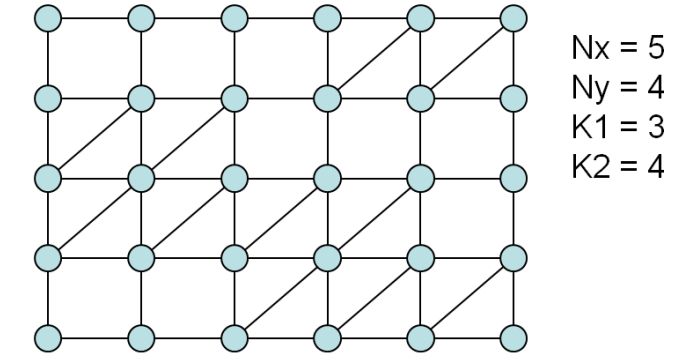
\includegraphics[width=85mm]{grid} \\
	\caption{Пример сетки для генерации графа} 
	\label{fig:grid}
\end{figure}

\newpage

\subsection{Краткое описание программной реализации}

...

\subsubsection{Запуск программы}

Для запуска на локальных системах достаточно указать количество нитей, а также все необходимые входные данные:

\begin{lstlisting}{bash}
	OMP_NUM_THREADS=k ./CGSolver Nx Ny K1 K2
\end{lstlisting}

Для запуска на кластере, использующем систему очередей, запускается скрипт со следующими параметрами:

\begin{lstlisting}{bash}
	mpisubmit.pl -t k CGSolver -- Nx Ny K1 K2
\end{lstlisting}

Однако желательно редактирование командного файла для запуска на заданных узлах и привязки к определенному сокету узла.

\begin{lstlisting}{bash}
	source /polusfs/setenv/setup.SMPI
	#BSUB -W 00:15
	#BSUB -o CGSolver.%J.out
	#BSUB -e CGSolver.%J.err
	#BSUB -m polus-c4-ib
	#BSUB -R affinity[core(10):distribute=pack(socket=1)]
	OMP_NUM_THREADS=k
	/polusfs/lsf/openmp/launchOpenMP.py CGSolver Nx Ny K1 K2
\end{lstlisting}


\newpage

\section{Исследование производительности}

\subsection{Характеристики вычислительной системы}

\begin{center}
	\setlength{\tabcolsep}{30pt}
	\renewcommand{\arraystretch}{1.5}
	\begin{tabular}{ c|c|c } 
		 & PC & Polus \\ 
		\hline
		CPU  & i5-12400F & IBM POWER 8 \\ 
		Cores & 6 & 10 \\ 
		Threads & 2 & 8 \\
		TPP & 384 GFLOPS & 290 GFLOPS \\
		RAM & 2xDDR5-5600  & 4xDDR4-2400 \\
		BW & 89.6 GB/s & 153.6 GB/s \\
	\end{tabular}
\end{center}

Для того, чтобы собрать программу и скомпилировать все файлы, необходимо выполнить ряд следующих действий:

\begin{lstlisting}{bash}
	mkdir build && cd build
	cmake -DENABLE_TESTS=<On|Off> -DUSE_DEBUG_MODE=<On|Off> ..
	make -j 4
	cd ../bin
\end{lstlisting}

Также на локальных системах можно запустить несколько простых тестов для проверки корректности работы программы (при условии, что на этапе сборки флаг ENABLE\_TESTS был включен):

\begin{lstlisting}{bash}
	cd build/Tests
	ctest
\end{lstlisting}


\subsection{Результаты измерений производительности}

\subsubsection{Последовательная производительность}

\begin{figure}[H]
	\center
	\begin{tabular}{cc}
		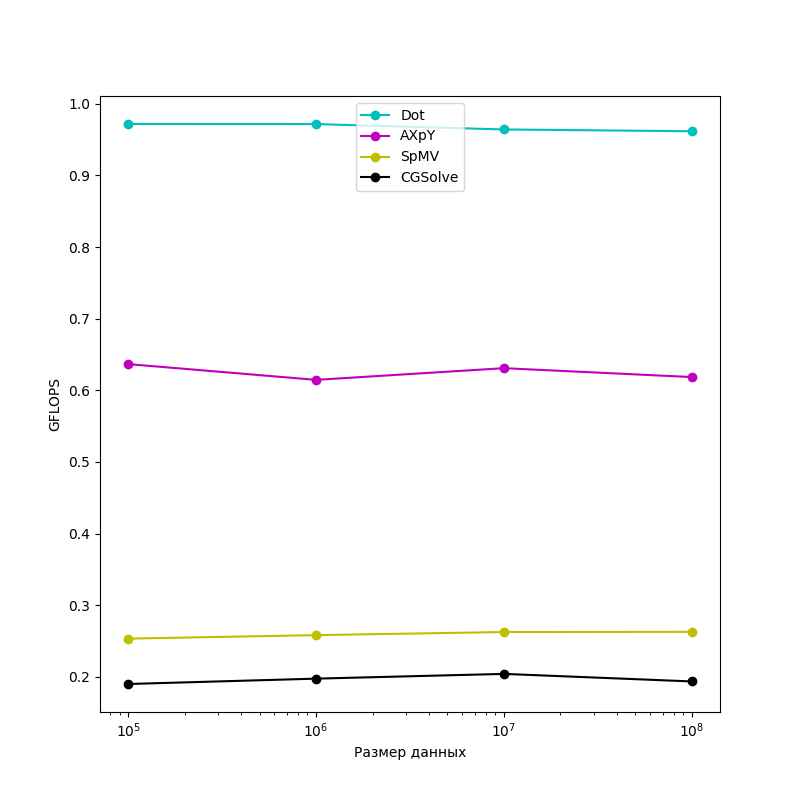
\includegraphics[width=85mm]{singlethread_pc} & 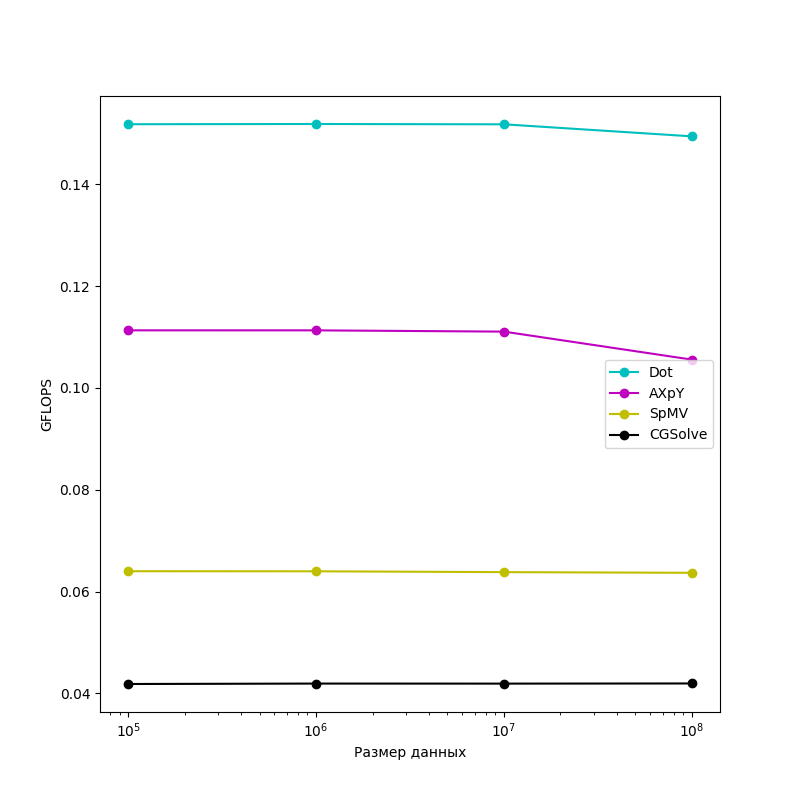
\includegraphics[width=85mm]{singlethread_polus} \\
		(а) PC & (б) Polus \\[6pt]
	\end{tabular}
	\caption{Зависимость производительности от размера входных данных} 
	\label{fig:singlethread_flops}
\end{figure}

\begin{figure}[H]
	\center
	\begin{tabular}{cc}
		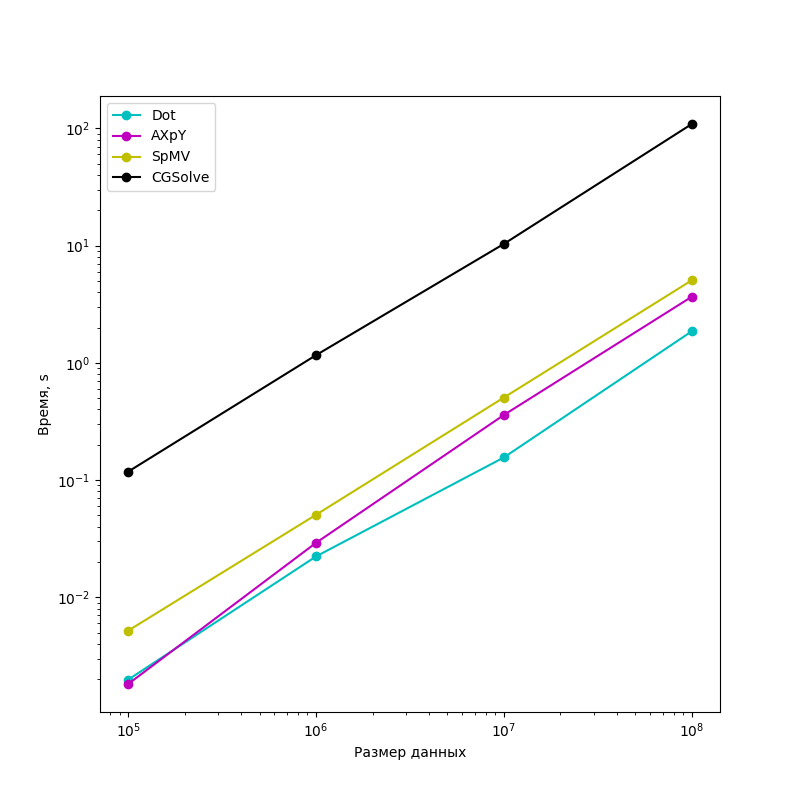
\includegraphics[width=85mm]{singlethread_time} & 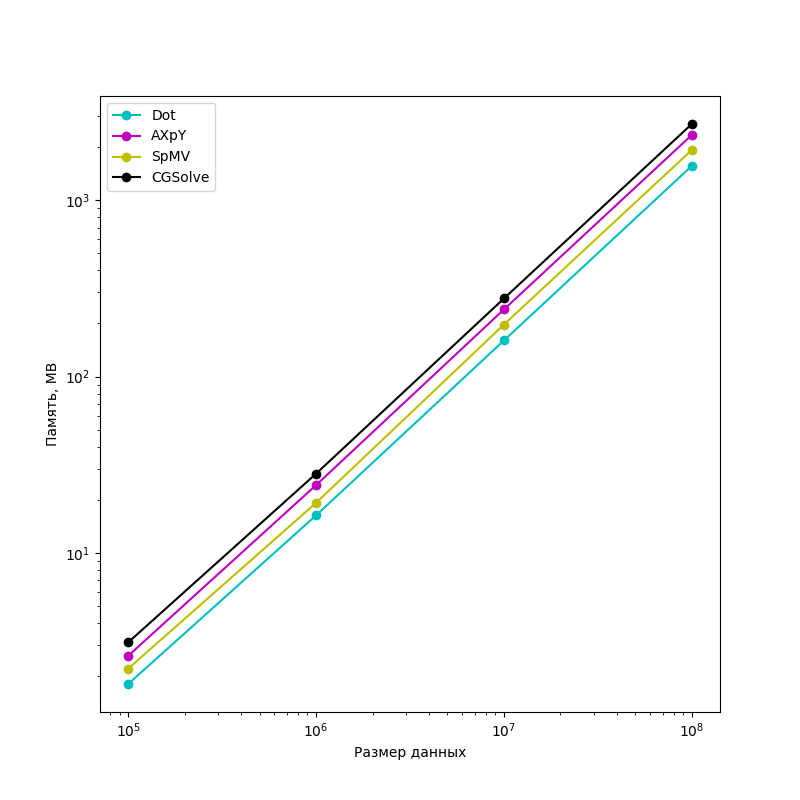
\includegraphics[width=85mm]{singlethread_memory} \\
		(а) & (б) \\[6pt]
	\end{tabular}
	\caption{Зависимость времени выполнения (а) и выделяемой памяти (б) в зависимости от размера входных данных}
	\label{fig:singlethread_time_memory}
\end{figure}

\subsubsection{Параллельное ускорение}

\begin{figure}[H]
	\center
	\begin{tabular}{cc}
		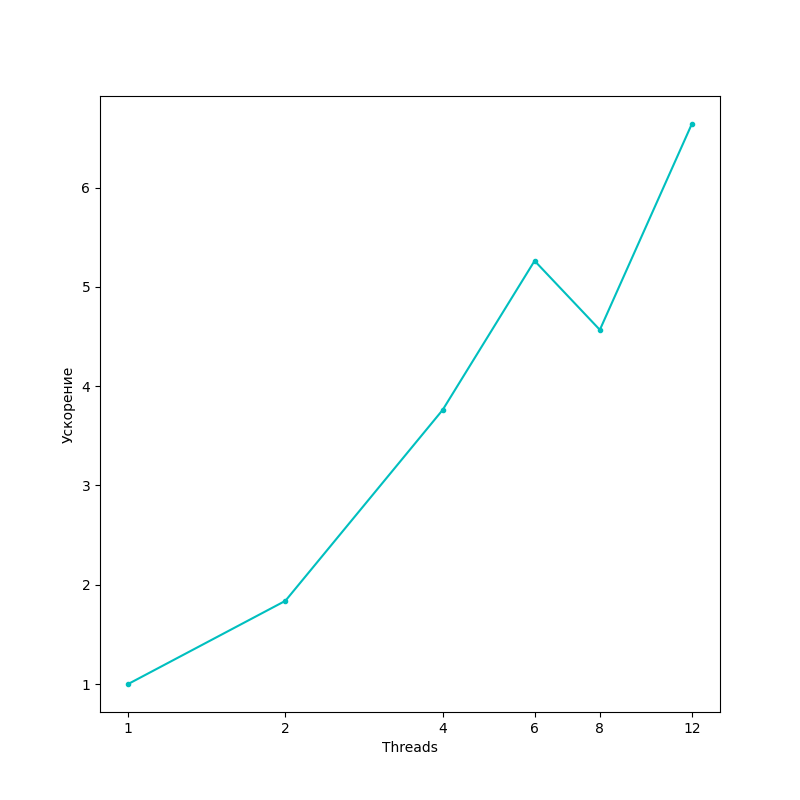
\includegraphics[width=85mm]{csr_init_speedup} & 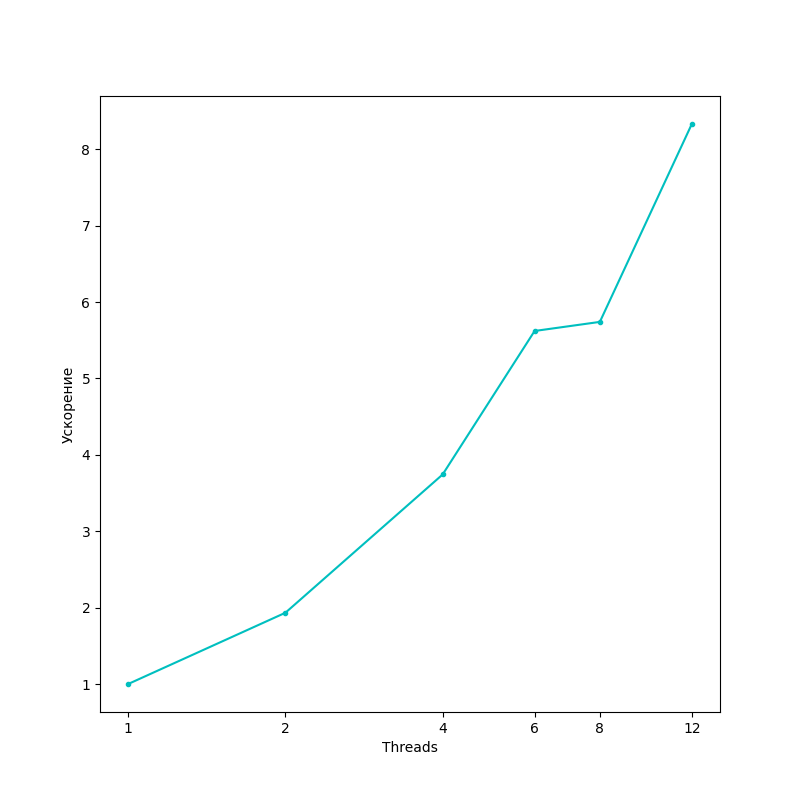
\includegraphics[width=85mm]{csr_fill_speedup} \\
		(а) & (б) \\[6pt]
	\end{tabular}
	\caption{Зависимость времени создания (а) и заполнения (б) массивов формата CSR в зависимости от числа нитей} 
	\label{fig:gridd}
\end{figure}

\begin{figure}[H]
	\center
	\begin{tabular}{cc}
		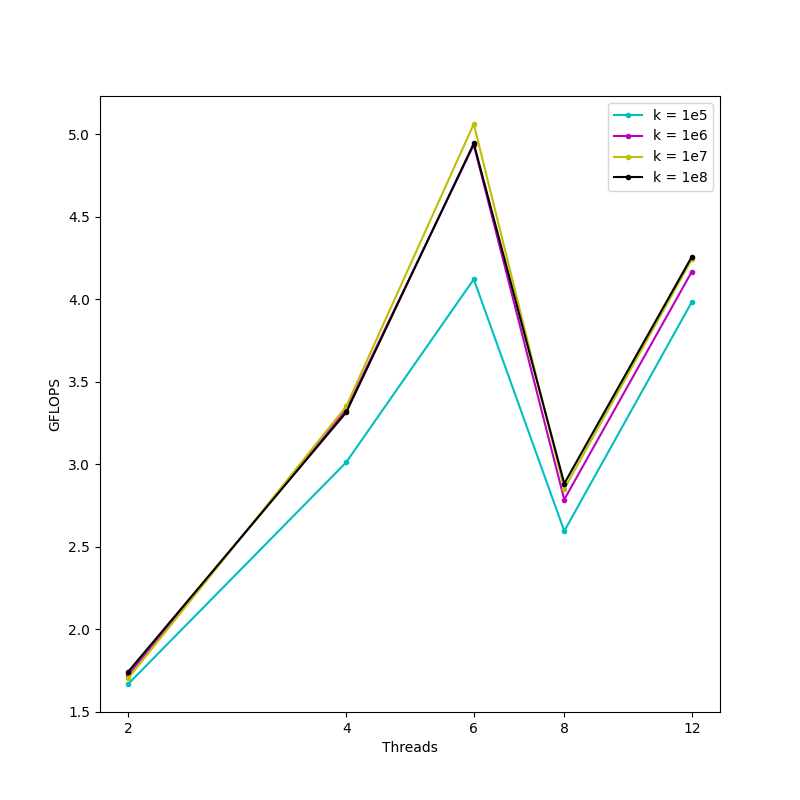
\includegraphics[width=85mm]{multithread_pc_dot} & 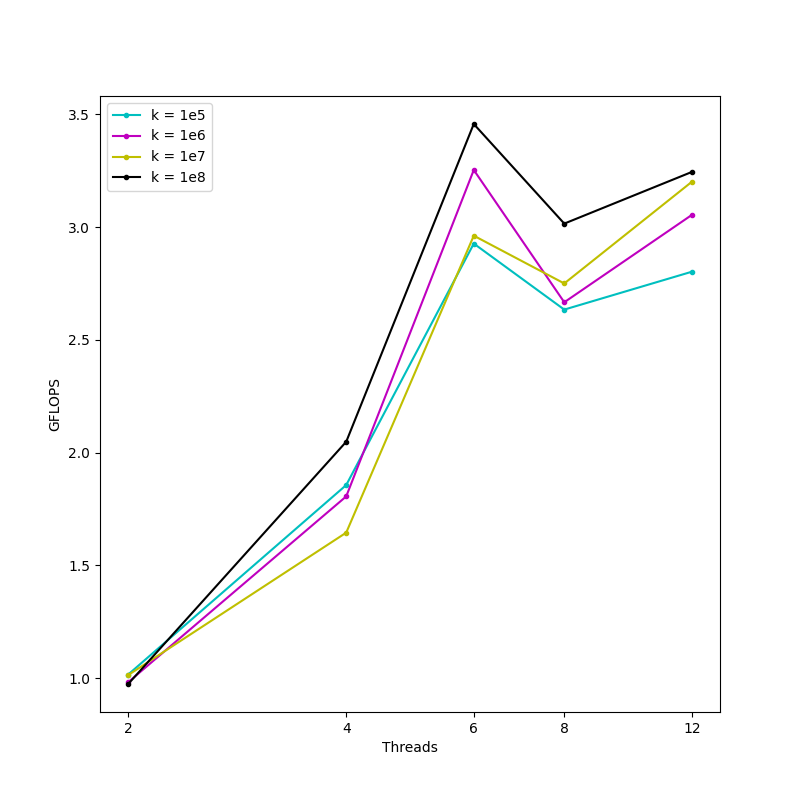
\includegraphics[width=85mm]{multithread_pc_axpy} \\
		(a) Dot & (б) AXpY \\
		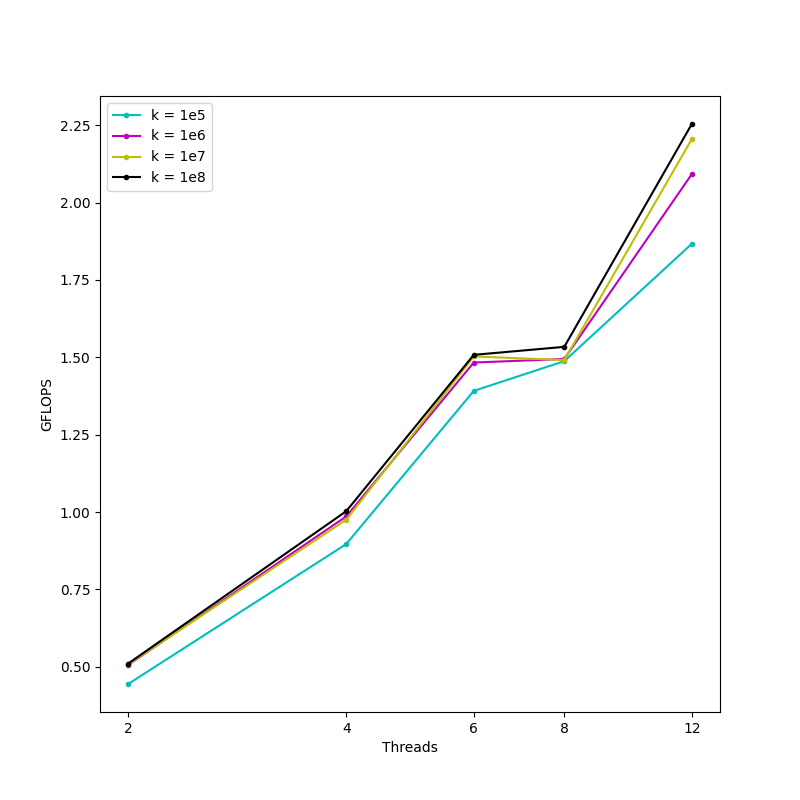
\includegraphics[width=85mm]{multithread_pc_spmv} & 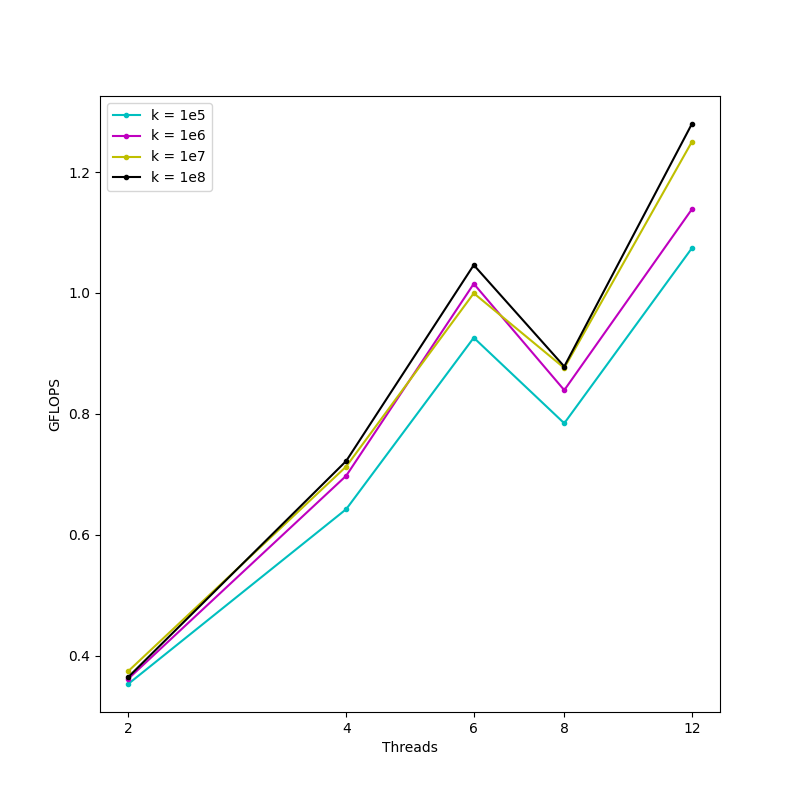
\includegraphics[width=85mm]{multithread_pc_cgsolver} \\
		(в) SpMV & (г) CGSolver \\[6pt]
	\end{tabular}
	\caption{Зависимость производительности от числа нитей (PC)}
	\label{fig:multithread_flops_pc} 
\end{figure}

\begin{figure}[H]
	\center
	\begin{tabular}{cc}
		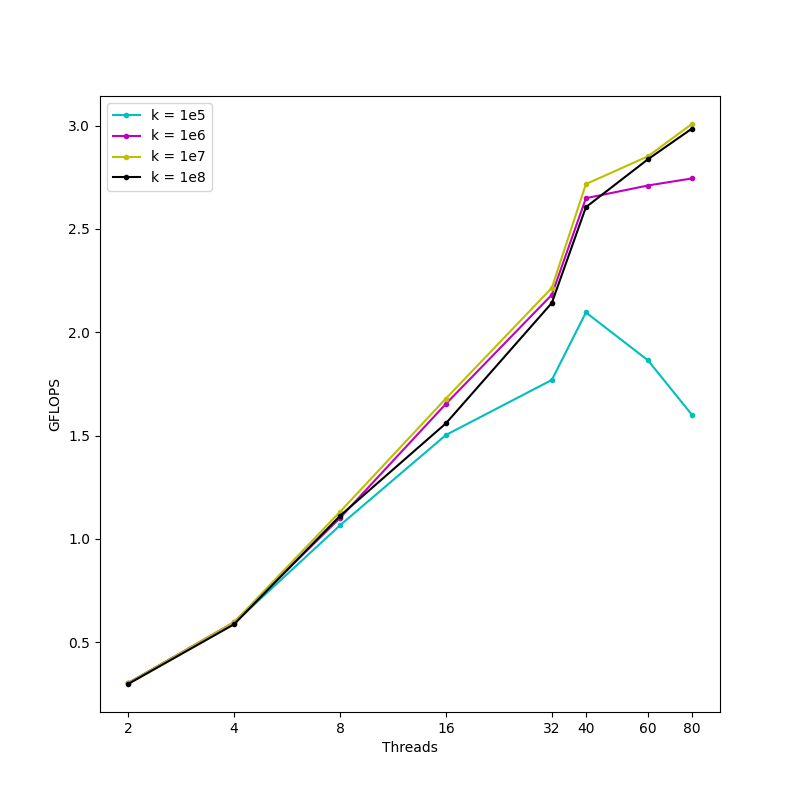
\includegraphics[width=85mm]{multithread_polus_dot} & 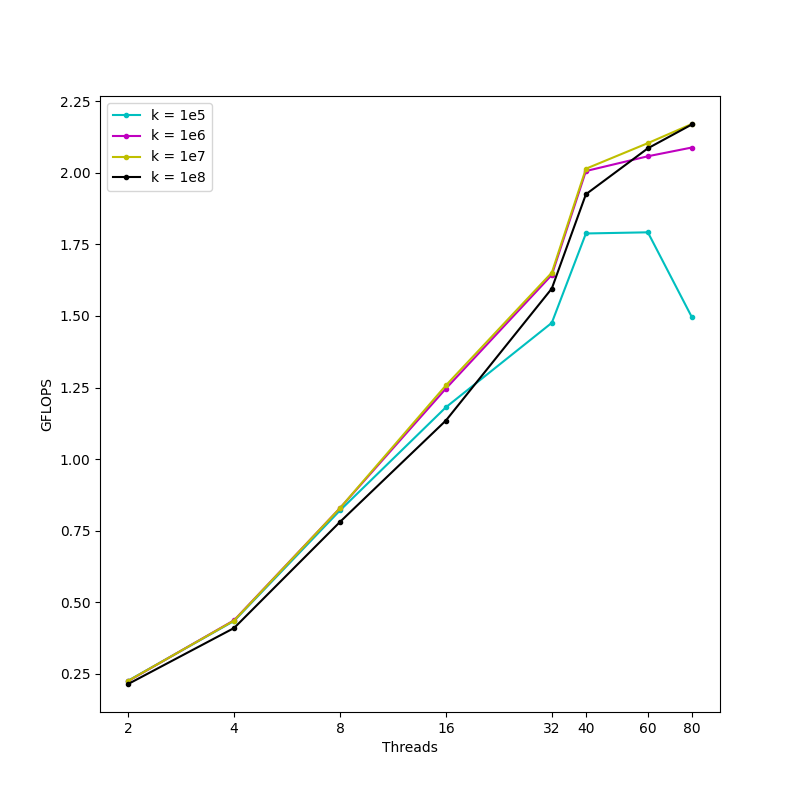
\includegraphics[width=85mm]{multithread_polus_axpy} \\
		(a) Dot & (б) AXpY \\
		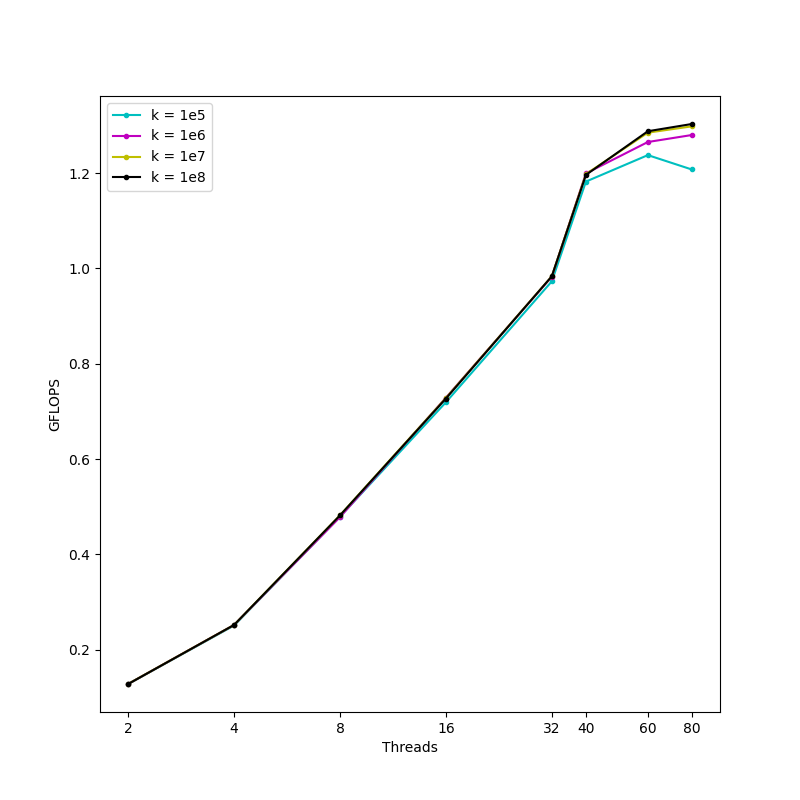
\includegraphics[width=85mm]{multithread_polus_spmv} & 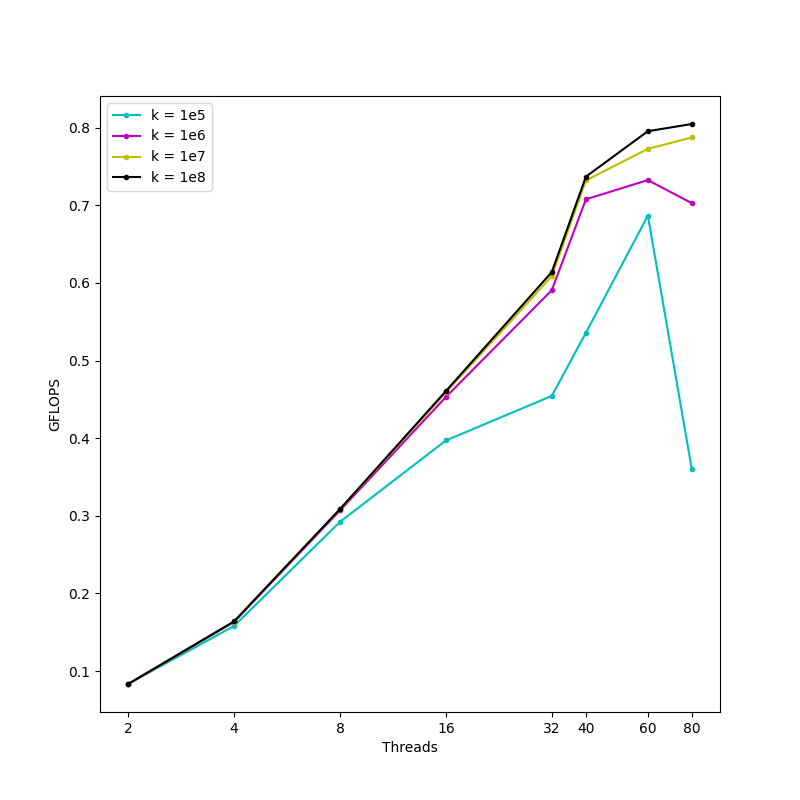
\includegraphics[width=85mm]{multithread_polus_cgsolver} \\
		(в) SpMV & (г) CGSolver \\[6pt]
	\end{tabular}
	\caption{Зависимость производительности от числа нитей (Polus)}
	\label{fig:multithread_flops_polus} 
\end{figure}

\begin{figure}[H]
	\center
	\setlength{\tabcolsep}{10pt}
	\renewcommand{\arraystretch}{1.5}
	\begin{tabular}{|c|c|c|c|c|c|c|c|c|}
		\hline
		T & 2 & 4 & 8 & 16 & 32 & 40 & 64 & 80  \\
		\hline
		Dot & 1.99 & 3.92 & 7.44 & 10.43 & 14.34 & 17.44 & 18.99 & 19.98 \\
		\hline
		AXpY & 2.04 & 3.89 & 7.40 & 10.75 & 15.12 & 18.24 & 19.76 & 20.55  \\
		\hline
		SpMV & 2.01 & 3.96 & 7.57 & 11.42 & 15.45 & 18.79 & 20.23 & 20.46  \\
		\hline
		CGSolve & 1.99 & 3.91 & 7.36 & 10.98 & 14.64 & 17.56 & 18.96 & 19.18 \\
		\hline
	\end{tabular}
	\caption{Расчеты ускорения для каждой из операций при $N = 1e8$ (Polus)}
	\label{fig:speedup}
\end{figure}

\newpage

\section{Анализ полученных результатов}

$ TPP_{PC} = 4\ GHz \cdot 6\ Cores \cdot 2\ Threads/Core \cdot 512/64 = 384\ GFLOPS $ 

$ TPP_{Polus} = 290\ GFLOPS $

$ BW_{PC} = 2\ Channels \cdot 5600\ MT/s \cdot 8\ bytes = 89,6\ GB/s $

$ BW_{Polus} = 8\ Channels \cdot 2400\ MT/s \cdot 8\ bytes = 153,6\ GB/s $ \\ \\

$ AI_{dot} = 2\ FLOP / (2 \cdot 8)\ bytes = 1/8 $

На каждой итерации считываем из памяти $x[i]$ и $y[i]$, каждый из которых типа 'double' занимает --- 8 байт. При этом на каждой итерации происходит 2 операции: умножение $x[i] \cdot y[i]$ и сложение с итоговой суммой

$ AI_{AXpY} = 2\ FLOP / (3 \cdot 8)\ bytes = 1/12 $

На каждой итерации считываем из памяти $x[i]$ и $y[i]$, каждый из которых типа 'double' занимает --- 8 байт, а также записываем в память результат $z[i] = a \cdot x[i] + y[i]$ типа 'double' --- тоже 8 байт. Следовательно, всего $3 \cdot 8$ байтов. При этом на каждой итерации происходит 2 операции: умножение $a \cdot x[i]$ и сложение $x[i] + y[i]$

$ AI_{SpMV} = 12\ FLOP / (132)\ bytes = 1/11 $ 

За итерацию будем считать умножение строки $i$ матрицы $A$ на столбец $x$. Для считывания элементов матрицы $A$ необходимо вначале получить номер $col=ia[i]$, с которого в массиве $a$ начинают храниться элементы $i$-ой строки --- 4 байта ($ia$ имеет тип 'int'). Далее будем считать, что в среднем в строке 6 ненулевых элементов. Для каждого такого элемента необходимо считать значение $a[col]$ типа 'double' --- 8 байт, считать $j = ja[col]$ номер столбца --- 4 байта ($ja$ имеет тип 'int'), а также считать $x[j]$ типа 'double' --- 8 байт. В конце вычислений необходимо записать полученный результат в $y[i]$ типа 'double' --- 8 байт. Таким образом получаем, что на каждую строку нам понадобится $4 + 6 \cdot (4 + 8 + 8) + 8 = 132$. При этом для каждого элемента строки потребуется 2 операции (умножение $a[col] \cdot x[j]$ и сложение в общий результат). Следовательно всего $6 \cdot 2 = 12$ операций.
 \\ \\ 


$ TBP = \min(TPP, BW \cdot AI)  $

$ TBP_{PC, dot} = \min(384\ GFLOPS, 89,6\ GB/s \cdot 1/8) = 11.2\ GFLOPS $

$ TBP_{PC, AXpY} = \min(384\ GFLOPS, 89,6\ GB/s \cdot 1/12) = 7.5\ GFLOPS $

$ TBP_{PC, SpMV} = \min(384\ GFLOPS, 89,6\ GB/s \cdot 1/11) = 8.1\ GFLOPS $

$ TBP_{Polus, dot} = \min(290\ GFLOPS, 153,6\ GB/s \cdot 1/8) = 19.2\ GFLOPS $

$ TBP_{Polus, AXpY} = \min(290\ GFLOPS, 153,6\ GB/s \cdot 1/12) = 12.8\ GFLOPS $

$ TBP_{Polus, SpMV} = \min(290\ GFLOPS, 153,6\ GB/s \cdot 1/11) = 14\ GFLOPS $

\begin{figure}[h!]
	\center
	\setlength{\tabcolsep}{10pt}
	\renewcommand{\arraystretch}{1.5}
	\begin{tabular}{|l|c|c|c|}
		\hline
		... & Dot & AXpY & SpMV \\
		\hline
		$PC\ TBP_{Analytical} $ & $ 11.2\ GFLOPS $ & $ 7.5\ GFLOPS $ & $ 8.1\ GFLOPS $ \\
		\hline
		$PC\ RealP $ & $ 5.06\ GFLOPS $ & $ 3.45\ GFLOPS $ & $ 2.25\ GFLOPS $ \\
		\hline
		$ Polus\ TBP_{Analytical} $& $ 19.2\ GFLOPS $ & $ 12.8\ GFLOPS $ & $ 14\ GFLOPS $ \\
		\hline
		$ Polus\ RealP $ & $ 3.01\ GFLOPS $ & $ 2.16\ GFLOPS $ & $ 1.31\ GFLOPS $ \\
		\hline
	\end{tabular}
	\caption{Аналитические и реальные значение производительности для каждой из операций}
	\label{fig:tbps}
\end{figure}

\end{document}